
          %-------------------%
\chapter{~~General description}\label{\numb section 1}
          %-------------------%

This section is a quick tour through \maniFEM's capabilities.


          %---------------------%
\section{~~An elementary example}\label{\numb section 1.\numb parag 1}
          %---------------------%

In this paragraph, we show how to build a rectangular mesh on a surface in $ \mathbb{R}^3 $ 
and then compute the integral of a given function.
Paragraph \ref{\numb section 1.\numb parag 4} shows a purely two-dimensional example.

\begin{figure} \centering
  \psfrag{SW}{\small\tt\textcolor{textindraw}{SW}}
  \psfrag{NW}{\small\tt\textcolor{textindraw}{NW}}
  \psfrag{SE}{\small\tt\textcolor{textindraw}{SE}}
  \psfrag{NE}{\small\tt\textcolor{textindraw}{NE}}
  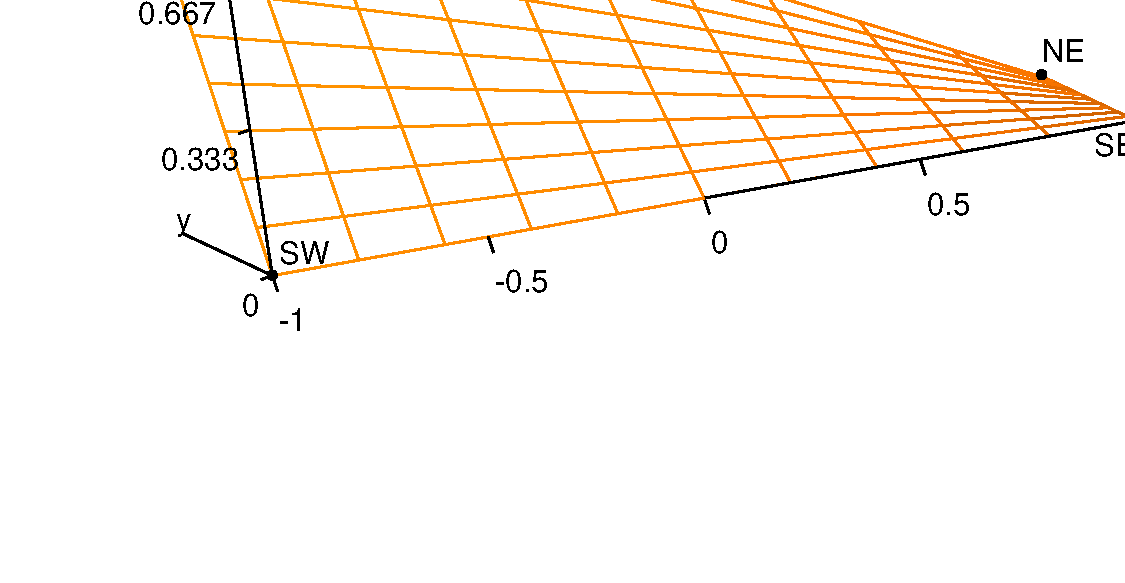
\includegraphics[width=95mm]{3d-rectangle}
  \caption{A twisted rectangular mesh}
  \label{\numb section 1.\numb fig 1}
\end{figure}

\begin{Verbatim}[commandchars=\\\{\},formatcom=\small\tt,frame=single,
   label=parag-\ref{\numb section 1.\numb parag 1}.cpp,rulecolor=\color{coment},
   baselinestretch=0.94,framesep=2mm                                            ]
#include \verde{"maniFEM.h"}

using namespace \verm{maniFEM};
using namespace std;

int main ()

\{  \cinza{// we choose our (geometric) space dimension :}
   \verm{Manifold} \azul{RR3} ( \textcolor{tag}{tag}::Euclid, \textcolor{tag}{tag}::of_dim, \laranja{3} );
   
   \cinza{// xyz is a map defined on our future mesh with values in RR3 :}
   \verm{Function} \azul{xyz} = RR3 .build_coordinate_system ( \textcolor{tag}{tag}::Lagrange, \textcolor{tag}{tag}::of_degree, \laranja{1} );

   \cinza{// we can extract components of xyz using the [] operator}
   \verm{Function} \azul{x} = xyz [\laranja{0}], \azul{y} = xyz [\laranja{1}], \azul{z} = xyz [\laranja{2}];

   \cinza{// Let's build a rectangular mesh. First, the four corners :}
   \verm{Cell} \azul{SW} ( \textcolor{tag}{tag}::vertex );  x (SW) = \laranja{-1};  y (SW) = \laranja{0};  z (SW) = \laranja{0};
   \verm{Cell} \azul{SE} ( \textcolor{tag}{tag}::vertex );  x (SE) =  \laranja{1};  y (SE) = \laranja{0};  z (SE) = \laranja{0};
   \verm{Cell} \azul{NE} ( \textcolor{tag}{tag}::vertex );  x (NE) =  \laranja{1};  y (NE) = \laranja{1};  z (NE) = \laranja{0};
   \verm{Cell} \azul{NW} ( \textcolor{tag}{tag}::vertex );  x (NW) = \laranja{-1};  y (NW) = \laranja{1};  z (NW) = \laranja{1};
   
   \cinza{// we access the coordinates of a point using the () operator :}
   cout << \verde{"coordinates of NW : "} << x (NW) << \verde{" "} << y (NW) << \verde{" "} << z (NW) << endl;
   \cinza{// now build the four sides of the rectangle :}
   \verm{Mesh} \azul{south} ( \textcolor{tag}{tag}::segment, SW .reverse(), SE, \textcolor{tag}{tag}::divided_in, \laranja{10} );
   \verm{Mesh} \azul{east}  ( \textcolor{tag}{tag}::segment, SE .reverse(), NE, \textcolor{tag}{tag}::divided_in, \laranja{10} );
   \verm{Mesh} \azul{north} ( \textcolor{tag}{tag}::segment, NE .reverse(), NW, \textcolor{tag}{tag}::divided_in, \laranja{10} );
   \verm{Mesh} \azul{west}  ( \textcolor{tag}{tag}::segment, NW .reverse(), SW, \textcolor{tag}{tag}::divided_in, \laranja{10} );
   
   \cinza{// and now the rectangle :}
   \verm{Mesh} \azul{rect_mesh} ( \textcolor{tag}{tag}::rectangle, south, east, north, west );

   \cinza{// We may want to visualize the resulting mesh.}
   \cinza{// Here is one way to export the mesh in the "msh" format :}
   rect_mesh .export_msh (\verde{"rectangle.msh"});

   \cinza{// Let's define a symbolic function to integrate}
   \verm{Function} \azul{f} = x*x + \laranja{1}/(\laranja{5}+y);
   \cinza{// and compute its integral on the rectangle,}
   \cinza{// using Gauss quadrature with 9 points}

   \verm{FiniteElement} \azul{fe}
      ( \textcolor{tag}{tag}::with_master, \textcolor{tag}{tag}::quadrangle, \textcolor{tag}{tag}::Lagrange, \textcolor{tag}{tag}::of_degree, \laranja{1} );
   fe .set_integrator ( \textcolor{tag}{tag}::Gauss, \textcolor{tag}{tag}::quad_9 );

   \cinza{// code below does not work yet}

   \cinza{// cout << "integral of " << f.repr() << " = "}
   \cinza{//      << fe .integrate ( f, tag::over, rect_mesh ) << endl;}
   \cinza{// cout << "integral of " << g.repr() << " = "}
   \cinza{//      << fe .integrate ( g, tag::over, rect_mesh ) << endl;}

\}  \cinza{// end of main}
\end{Verbatim}

Paragraph \ref{\numb section 11.\numb parag 2} explains the coloring conventions observed
in this manual for {\tt C++} code.

To run this example, you will need a recent {\tt C++} compiler and the {\tt make} utility.
Visit {\small\tt https://github.com/cristian-barbarosie/manifem}, choose a release
and download all files to some directory in your computer.
Paragraph \ref{\numb section 11.\numb parag 16} gives more details.
% Latest code may be unstable, releases are stable.
Launch the program through the command
{\small\tt make run-\ref{\numb section 1.\numb parag 1}};
a file {\small\tt rectangle.msh} should appear in the working directory.
You may view the mesh using the software {\tt gmsh}.

Expressions like {\small\tt \textcolor{tag}{tag}::of\_\,dim} and {\small\tt \textcolor{tag}{tag}::vertex} are
objects belonging to the {\small\tt namespace \textcolor{tag}{tag}};
we use them as arguments to many functions.
See paragraph \ref{\numb section 11.\numb parag 3} for some details.

When declaring a segment {\small\tt \verm{Mesh}}, we must {\small\tt reverse} the first vertex
(paragraph \ref{\numb section 1.\numb parag 2} discusses the {\small\tt reverse} method).
Paragraph \ref{\numb section 1.\numb parag 4} explains why we build
the rectangle based on its four sides rather than on its four vertices.

Note that in this example we do not have exact control on the shape of the surface being meshed.
The coordinates of the inner vertices are defined rather vaguely by interpolating the
coordinates of the four corners.
See sections \ref{\numb section 2} and \ref{\numb section 3} for ways to precisely define
a submanifold in $ \mathbb{R}^3 $ and mesh (a bounded domain of) it.


          %----------------%
\section{~~Cells and meshes}\label{\numb section 1.\numb parag 2}
          %----------------%

In \maniFEM, all basic constituents of meshes are called ``cells''. 
Points are zero-dimensional cells, segments are one-dimensional cells, triangles are
two-dimensional cells, and so on.

Roughly speaking, a mesh is a collection of cells of the same dimension. 
For efficiency reasons, meshes keep lists of cells of lower dimension, too. 
For instance, the mesh built in paragraph \ref{\numb section 1.\numb parag 1} is 
roughly a list of two-dimensional cells (quadrilaterals), but lists of segments and points
are also kept.
This represents quite some amount of redundant information, but it is useful e.g.\ for
quickly sweeping over all vertices of a mesh.%
\footnote {Actually, the implementation details are more complicated.
There are different kinds of meshes, some of them keep more information (lists of cells)
and are faster; others are slower but lighter in terms of memory occupied.
See e.g. paragraph \ref{\numb section 11.\numb parag 6}.}

A cell of dimension $ d>0 $ is defined by its boundary, 
which in turn is a mesh of dimension $ d-1 $. 
The boundary of a segment is a (zero-dimensional) mesh made of two points.
The boundary of a triangle is a one-dimensional mesh made of three segments.
Thus, a segment is essentially a pair of points, a triangle is essentially a triplet of segments, and so on.

Cells and meshes are oriented. 
An orientation of a mesh is just an orientation for each of its component cells
(of course these orientations must be mutually compatible).
Although this is not how the orientation is implemented internally
(see paragraph \ref{\numb section 11.\numb parag 4}),
an oriented point can be conceived simply as a point with a sign attached (1 or -1). 
The orientation of a cell of dimension higher than zero is given by an orientation
of its boundary, which is a lower-dimensional mesh.

Thus, an oriented segment is essentially a pair of points, one of which has a \hbox{-1}
attached, the other having a 1.
We call the former ``base'' and the latter ``tip''.
These signs are related to integration of functions along that segment.
The integral of a function of one variable is equal to the value of the 
primitive function at one end of the segment minus the value of the primitive at the other end.

An oriented triangle is essentially a triplet of segments, each one with its own orientation.
The orientations must be compatible to each other in the sense that each vertex 
must be seen as positive by one of the segments and as negative by another one.
An oriented tetrahedron can be identified with four triangles, each one with its own
orientation.
In such a tetrahedron, each segment must be seen as positive by one of the triangles and
as negative by another one.

\begin{figure}[ht] \centering
  \psfrag{A}{\small\tt\textcolor{textindraw}{A}}
  \psfrag{B}{\small\tt\textcolor{textindraw}{B}}
  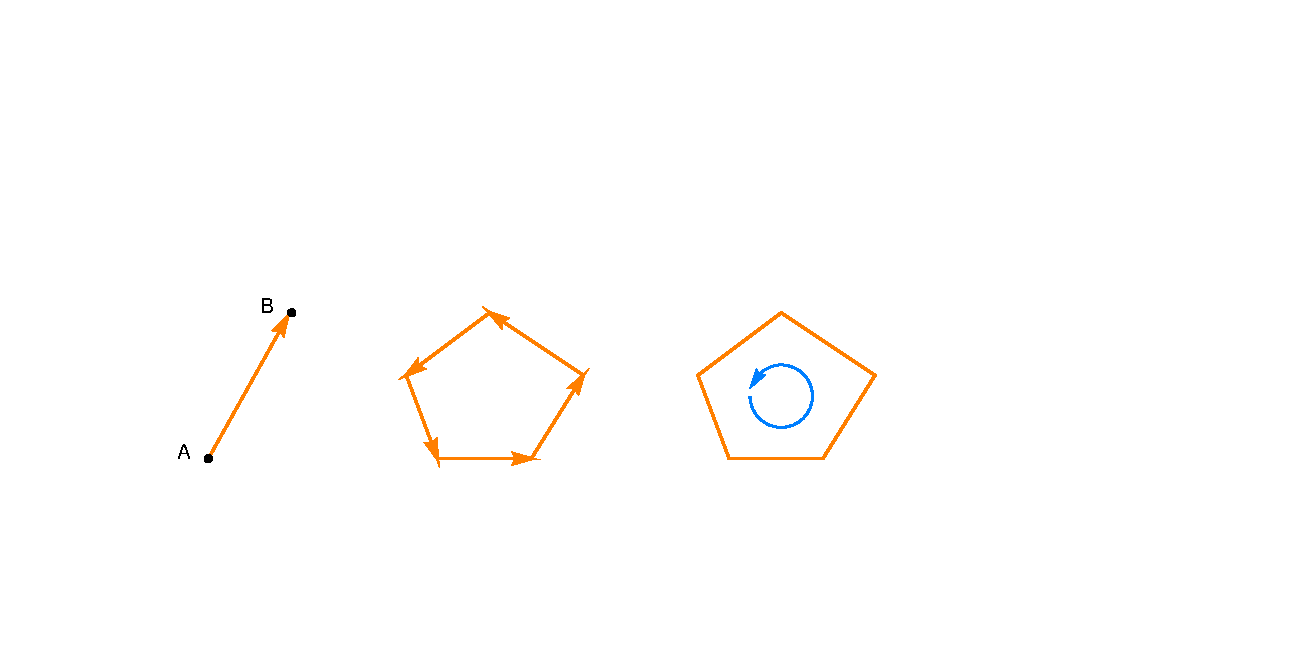
\includegraphics[width=90mm]{oriented-cells.eps}
  \caption{Oriented segment, oriented pentagon}
  \label{\numb section 1.\numb fig 2}
\end{figure}

We can think of an oriented segment as an arrow pointing from its negative extremity (base)
towards its positive extremity (tip).
We can think of an oriented polygon as having an arrow attached to each of it sides,
or we can imagine a small oriented circle inside the polygon.

\begin{figure} \centering
  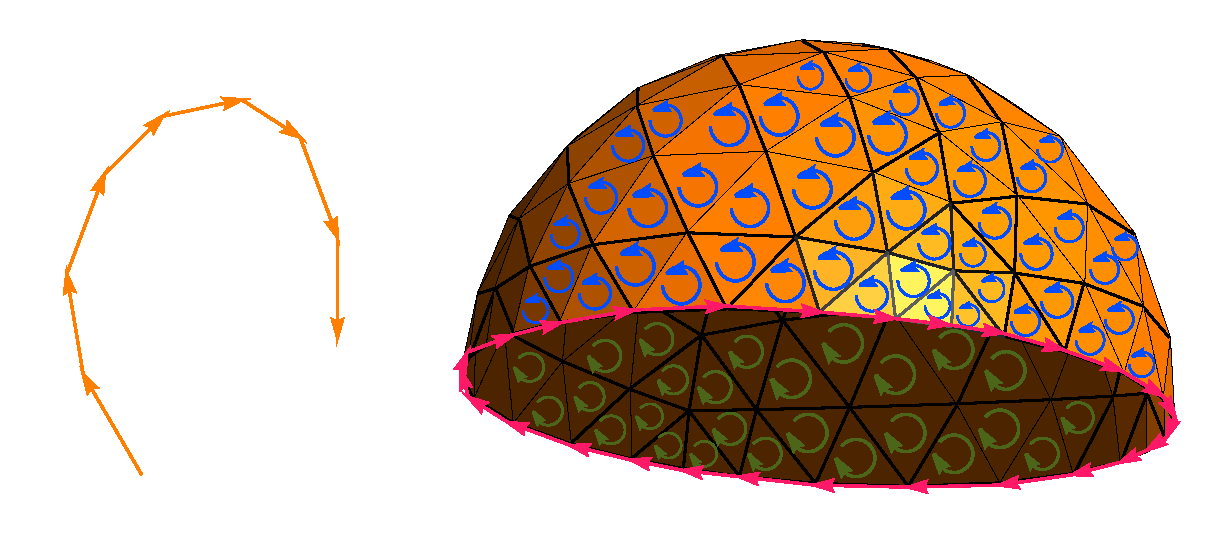
\includegraphics[width=125mm]{hemisphere-7}
  \caption{Oriented meshes of dimension one and two}
  \label{\numb section 1.\numb fig 3}
\end{figure}

A one-dimensional oriented mesh can be thought of as a chain of arrows,
each one pointing to the next segment's base (like in figure \ref{\numb section 1.\numb fig 3}
right).
A two-dimensional oriented triangular mesh can be thought of as a web of triangles,
each triangle having a small oriented circle inside (like in figure
\ref{\numb section 1.\numb fig 3} left).
The orientations of neighbour cells must be compatible : each segment must be seen
in opposite orientations from the point of view of its two neighbour triangles.

The above description of the orientation of a two-dimensional mesh does not depend
on the surrounding space.
A mesh can be immersed in some Euclidian space $ \mathbb{R}^d $ or not.
As an extreme example, vertices may even have no coordinates at all.
However, in the case of a two-dimensional mesh immersed in $ \mathbb{R}^3 $,
the right hand rule establishes a correspondence between the oriented circle described above
and an arrow normal to the surface being meshed.
Note that the right hand rule is a convention based on the assuption that
the surrounding space $ \mathbb{R}^3 $ has a certain orientation.

Note also that an orientation of a mesh defines an orientation of its boundary.
In figure \ref{\numb section 1.\numb fig 3} we can see the orientation of the
boundary of the mesh, shown with pink arrows.
This convention is used by Stokes' theorem.

Figure \ref{\numb section 1.\numb fig 4} shows two opposite orientations of a mesh,
together with the corresponding orientation of its boundary.

\begin{figure}[ht] \centering
\begin{subfigure}{76mm}\centering
  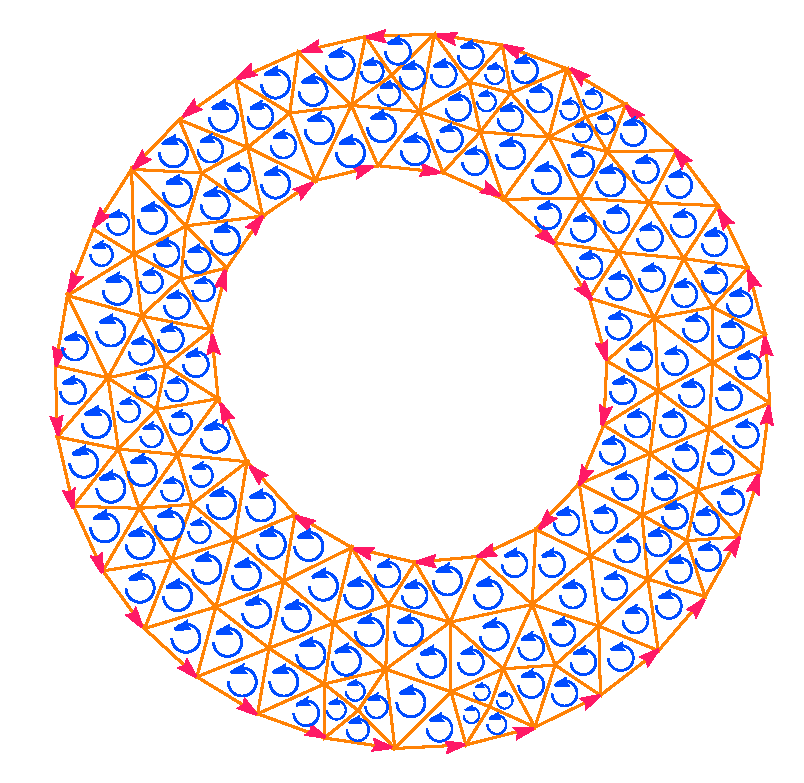
\includegraphics[width=75mm]{oriented-annulus-1}
\end{subfigure}  
\begin{subfigure}{76mm}\centering
  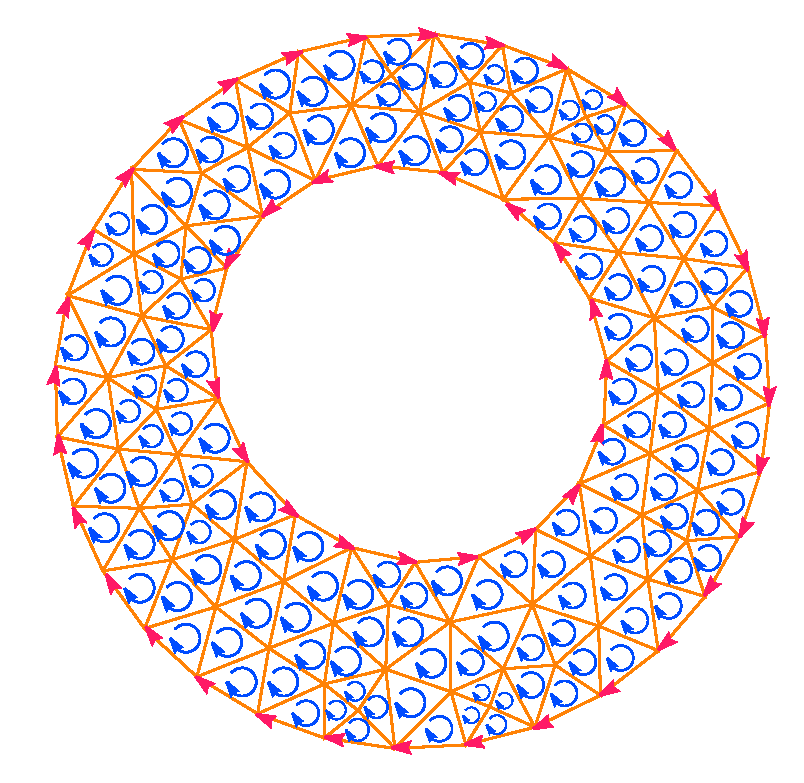
\includegraphics[width=75mm]{oriented-annulus-2}
\end{subfigure}  
  \caption{Mesh with two opposite orientations}
  \label{\numb section 1.\numb fig 4}
\end{figure}

Paragraphs \ref{\numb section 1.\numb parag 4} and \ref{\numb section 3.\numb parag 18}
show examples where the orientation of the boundary is important for joining meshes.
In progressive mesh generation (described in section \ref{\numb section 3}) we often
provide the boundary of the future mesh, whose orientation determines the output of the
algorithm.

Cells have a {\small\tt reverse} method returning the reversed cell.
Segment {\small\tt \verm{Cell}}s have methods {\small\tt base} and {\small\tt tip} returning their extremities.
For instance :

\begin{Verbatim}[commandchars=\\\{\},formatcom=\small\tt,baselinestretch=0.94]
   \verm{Cell} \azul{A} ( \textcolor{tag}{tag}::vertex );  \verm{Cell} \azul{B} ( \textcolor{tag}{tag}::vertex );
   assert ( A .is_positive() );
   assert ( not A .reverse() .is_positive() );
   assert ( A .reverse() .reverse() == A );
   \verm{Cell} \azul{AB} ( \textcolor{tag}{tag}::segment, A .reverse(), B );
   \cinza{// here, AB is a segment Cell, not a Mesh}
   assert ( AB .base() == A .reverse() );
   assert ( AB .tip() == B );

   \verm{Cell} \azul{BA} = AB .reverse();
   assert ( BA .base() == B .reverse() );
   assert ( BA .tip() == A );
   assert ( BA .reverse() == AB );
\end{Verbatim}

Paragraph \ref{\numb section 9.\numb parag 5} gives more details about the orientation of cells.
See also paragraph \ref{\numb section 11.\numb parag 4}.

Cells are topological entities; they carry no geometric information.
In particular, points do not have coordinates.
Coordinates are stored externally, see paragraph \ref{\numb section 5.\numb parag 1}.

{\small\tt \verm{Mesh}}es have a {\small\tt reverse} method, too.
It is used mainly when we want to {\small\tt join} meshes having a common piece of boundary;
see paragraphs \ref{\numb section 1.\numb parag 4}, \ref{\numb section 2.\numb parag 6},
\ref{\numb section 2.\numb parag 7}, \ref{\numb section 2.\numb parag 11},
\ref{\numb section 3.\numb parag 17}, \ref{\numb section 3.\numb parag 18}.


          %---------%
\section{~~Functions}\label{\numb section 1.\numb parag 3}
          %---------%

Minimalist programs like the pieces of code presented in paragraph
\ref{\numb section 1.\numb parag 2} work without declaring a {\small\tt\verm{Manifold}}
and without {\small\tt\verm{Function}}s.
However, any {\small\tt\verm{Mesh}} constructor will try to interpolate geometric coordinates
based on the shape of the current {\small\tt\verm{Manifold}}.

{\ManiFEM} uses {\small\tt\verm{Function}}s for several different purposes.
{\small\tt\verm{Function}}s can be divided roughly in two categories.
Some keep numeric values, like {\small\tt x}, {\small\tt y} and {\small\tt z}
encountered in many places in this manual.
After building such a function, for instance through the statement

\begin{Verbatim}[commandchars=\\\{\},formatcom=\small\tt,baselinestretch=0.94]
   \verm{Function} \azul{xyz} = RR3 .build_coordinate_system ( \textcolor{tag}{tag}::Lagrange, \textcolor{tag}{tag}::of_degree, \laranja{1} );
\end{Verbatim}

the process of creating a new vertex will change.
Space in the computer's memory will be reserved for {\small\tt d} values of type {\small\tt double}
({\small\tt d} being the dimension of the current {\small\tt\verm{Manifold}}) for each
new vertex.
{\small\tt\verm{Function}}s {\small\tt x}, {\small\tt y} and {\small\tt z} (components of
{\small\tt xyz}) are mere handlers through which we access these values.

Other {\small\tt\verm{Function}}s are not related with space in the computer's memory.
For instance, there are arithmetic expressions like 

\begin{Verbatim}[commandchars=\\\{\},formatcom=\small\tt,baselinestretch=0.94]
   \verm{Function} \azul{norm} = \verm{power} ( x*x + y*y + z*z, \laranja{0.5} );
\end{Verbatim}

We can still access the value of such a {\small\tt \verm{Function}} at a cell like in
{\small\tt double} {\small\tt \azul{n}} {\small\tt =} {\small\tt norm(A)};
the computer will return the value of the corresponding arithmetic expression,
replacing the symbols {\small\tt x}, {\small\tt y} and {\small\tt z} by the corresponding
values at cell {\small\tt A}.
But it makes no sense to change the value of {\small\tt norm} at cell {\small\tt A}.
Thus, pieces of code like {\small\tt x(A)} {\small\tt =} {\small\tt \laranja{1.}} work fine,
while {\small\tt norm(A)} {\small\tt =} {\small\tt \laranja{1.}} produces a run-time error.

The {\small\tt \verm{Function}::deriv} method performs symbolic differentiation :

\begin{Verbatim}[commandchars=\\\{\},formatcom=\small\tt,baselinestretch=0.94]
   \verm{Function} \azul{norm_x} = norm .deriv ( x );
   \verm{Function} \azul{norm_y} = norm .deriv ( y );
\end{Verbatim}


          %--------------%
\section{~~Joining meshes}\label{\numb section 1.\numb parag 4}
          %--------------%

The example in paragraph \ref{\numb section 1.\numb parag 1} could have been shortened
had we used the overloaded version of the {\small\tt \verm{Mesh}} constructor with
{\small\tt \textcolor{tag}{tag}::rectangle} which accepts the four corners as arguments. 
This overloaded version exists in \maniFEM, but we prefer to build meshes in a structured way, 
first corners, then sides and then the plane region. 
This has the advantage that one can build more complex meshes from simple components. 
For instance, one can build an L-shaped mesh by joining three rectangular meshes :

\begin{figure}[ht] \centering
  \psfrag{A}{\small\tt\textcolor{textindraw}{A}}
  \psfrag{B}{\small\tt\textcolor{textindraw}{B}}
  \psfrag{C}{\small\tt\textcolor{textindraw}{C}}
  \psfrag{D}{\small\tt\textcolor{textindraw}{D}}
  \psfrag{E}{\small\tt\textcolor{textindraw}{E}}
  \psfrag{F}{\small\tt\textcolor{textindraw}{F}}
  \psfrag{G}{\small\tt\textcolor{textindraw}{G}}
  \psfrag{H}{\small\tt\textcolor{textindraw}{H}}
  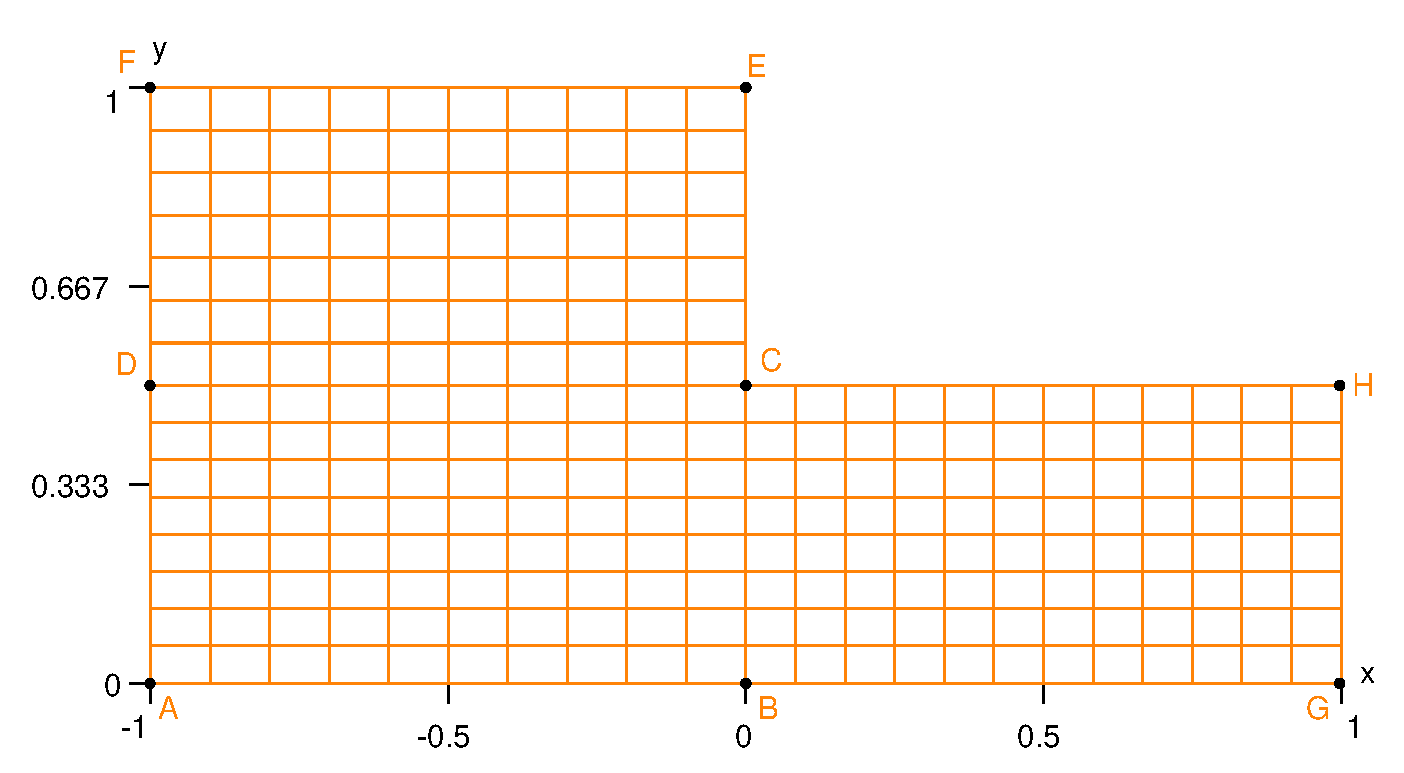
\includegraphics[width=115mm]{L-shaped}
  \caption{An L-shaped mesh}
  \label{\numb section 1.\numb fig 5}
\end{figure}

\begin{Verbatim}[commandchars=\\\{\},formatcom=\small\tt,frame=single,
   label=parag-\ref{\numb section 1.\numb parag 4}.cpp,rulecolor=\color{coment},
   baselinestretch=0.94,framesep=2mm]
   \verm{Manifold} \azul{RR2} ( \textcolor{tag}{tag}::Euclid, \textcolor{tag}{tag}::of_dim, \laranja{2} );
   \verm{Function} \azul{xy} = RR2 .build_coordinate_system ( \textcolor{tag}{tag}::Lagrange, \textcolor{tag}{tag}::of_degree, \laranja{1} );
   \verm{Function} \azul{x} = xy [\laranja{0}], \azul{y} = xy [\laranja{1}];

   \verm{Cell} \azul{A} ( \textcolor{tag}{tag}::vertex );  x (A) = \laranja{-1.};  y (A) = \laranja{0.};
   \verm{Cell} \azul{B} ( \textcolor{tag}{tag}::vertex );  x (B) =  \laranja{0.};  y (B) = \laranja{0.};
   \verm{Cell} \azul{C} ( \textcolor{tag}{tag}::vertex );  x (C) =  \laranja{0.};  y (C) = \laranja{0.5};
   \verm{Cell} \azul{D} ( \textcolor{tag}{tag}::vertex );  x (D) = \laranja{-1.};  y (D) = \laranja{0.5};
   \verm{Cell} \azul{E} ( \textcolor{tag}{tag}::vertex );  x (E) =  \laranja{0.};  y (E) = \laranja{1.};
   \verm{Cell} \azul{F} ( \textcolor{tag}{tag}::vertex );  x (F) = \laranja{-1.};  y (F) = \laranja{1.};
   \verm{Cell} \azul{G} ( \textcolor{tag}{tag}::vertex );  x (G) =  \laranja{1.};  y (G) = \laranja{0.};
   \verm{Cell} \azul{H} ( \textcolor{tag}{tag}::vertex );  x (H) =  \laranja{1.};  y (H) = \laranja{0.5};
   \verm{Mesh} \azul{AB} ( \textcolor{tag}{tag}::segment, A .reverse(), B, \textcolor{tag}{tag}::divided_in, \laranja{10} );
   \verm{Mesh} \azul{BC} ( \textcolor{tag}{tag}::segment, B .reverse(), C, \textcolor{tag}{tag}::divided_in,  \laranja{8} );
   \verm{Mesh} \azul{CD} ( \textcolor{tag}{tag}::segment, C .reverse(), D, \textcolor{tag}{tag}::divided_in, \laranja{10} );
   \verm{Mesh} \azul{DA} ( \textcolor{tag}{tag}::segment, D .reverse(), A, \textcolor{tag}{tag}::divided_in,  \laranja{8} );
   \verm{Mesh} \azul{CE} ( \textcolor{tag}{tag}::segment, C .reverse(), E, \textcolor{tag}{tag}::divided_in,  \laranja{7} );
   \verm{Mesh} \azul{EF} ( \textcolor{tag}{tag}::segment, E .reverse(), F, \textcolor{tag}{tag}::divided_in, \laranja{10} );
   \verm{Mesh} \azul{FD} ( \textcolor{tag}{tag}::segment, F .reverse(), D, \textcolor{tag}{tag}::divided_in,  \laranja{7} );
   \verm{Mesh} \azul{BG} ( \textcolor{tag}{tag}::segment, B .reverse(), G, \textcolor{tag}{tag}::divided_in, \laranja{12} );
   \verm{Mesh} \azul{GH} ( \textcolor{tag}{tag}::segment, G .reverse(), H, \textcolor{tag}{tag}::divided_in,  \laranja{8} );
   \verm{Mesh} \azul{HC} ( \textcolor{tag}{tag}::segment, H .reverse(), C, \textcolor{tag}{tag}::divided_in, \laranja{12} );

   \verm{Mesh} \azul{ABCD} ( \textcolor{tag}{tag}::rectangle, AB, BC, CD, DA );
   \verm{Mesh} \azul{CEFD} ( \textcolor{tag}{tag}::rectangle, CE, EF, FD, CD .reverse() );
   \verm{Mesh} \azul{BGHC} ( \textcolor{tag}{tag}::rectangle, BG, GH, HC, BC .reverse() );

   \verm{Mesh} \azul{L_shaped} ( \textcolor{tag}{tag}::join, ABCD, CEFD, BGHC );
\end{Verbatim}

Meshes in $ \mathbb{R}^2 $ like the one above may be exported in the {\small\tt msh} format
or directly drawn in {\small\tt PostScript}, by one of the two statements below

\begin{Verbatim}[commandchars=\\\{\},formatcom=\small\tt,baselinestretch=0.94]
   L_shaped .export_msh (\verde{"L-shaped.msh"});
   L_shaped .draw_ps (\verde{"L-shaped.eps"});
\end{Verbatim}

Note that, in \maniFEM, cells and meshes are oriented
(see paragraph \ref{\numb section 1.\numb parag 2}).
To build {\small\tt \azul{CEFD}} one must use not {\small\tt CD} but its reverse;
to build {\small\tt \azul{BGHC}} one must use not {\small\tt BC} but its reverse.
In figure \ref{\numb section 1.\numb fig 6} we see a zoom around {\small\tt C};
the three rectangular meshes have been separated just for visualization purposes.
The drawing illustrates that the common boundary has a certain orientation when seen
from one mesh and has the opposite orientation when seen from the neighbour mesh.
If we do not respect these orientations, {\maniFEM} will be unable to {\small\tt join}
these meshes.

\vskip 3mm plus 2mm
\begin{figure}[ht]  \centering
  \psfrag{C}{\small\tt\textcolor{textindraw}{C}}
  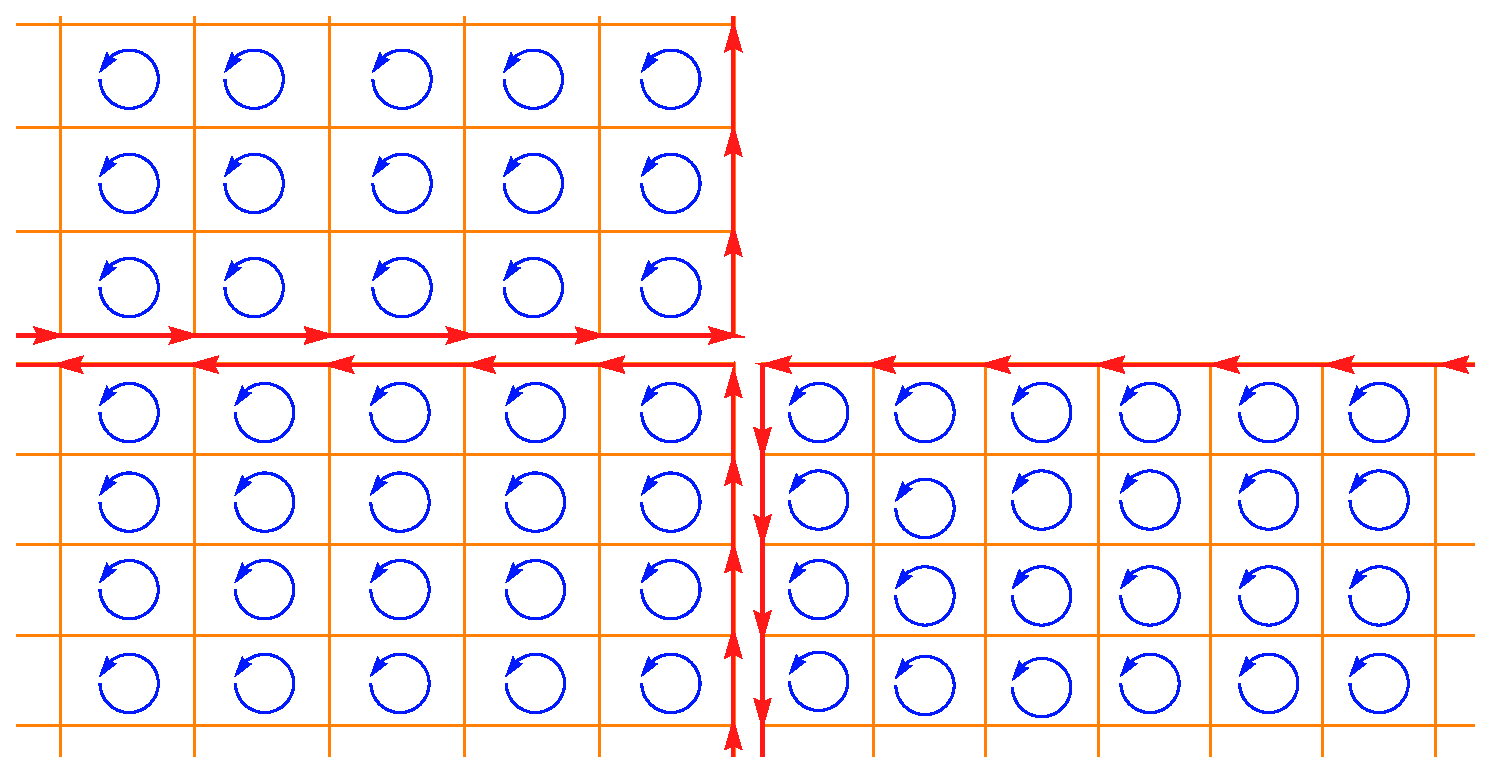
\includegraphics[width=120mm]{L-crack}
  \caption{A zoom around {\small\tt C}}
  \label{\numb section 1.\numb fig 6}
\end{figure}

We can imagine a magnet attached to each face of a cell.
For two neighbour cells, the common face will have two magnets, one from each cell.
If their polarities are not opposite, the magnets will not cling.
Likewise, the common boundary of two meshes that we intend to join can be thought of
as a pair of magnets.
If their polarities are not opposite, the two meshes will not cling.

Note also that if we define the rectangles based on their vertices instead of their sides, 
the {\small\tt \verm{Mesh}} constructor with {\small\tt \textcolor{tag}{tag}::join} will
not work properly. 
For instance, the two rectangles defined by

\begin{Verbatim}[commandchars=\\\{\},formatcom=\small\tt,baselinestretch=0.94]
   \verm{Mesh} \azul{ABCD} ( \textcolor{tag}{tag}::rectangle, A, B, C, D, \laranja{10}, \laranja{8} );
   \verm{Mesh} \azul{CEFD} ( \textcolor{tag}{tag}::rectangle, C, E, F, D, \laranja{7}, \laranja{10} );
\end{Verbatim}

\noindent cannot be joined%
\footnote {Actually, they can be joined but the resulting mesh will have
a crack along {\small\tt CD} -- probably not what the user wants.}
because the side {\small\tt CD} of {\small\tt ABCD} has nothing to do with the side 
{\small\tt DC} of {\small\tt CEFD}.
These two sides are one-dimensional meshes both made of 10 segments but with different
interior points (only {\small\tt C} and {\small\tt D} are shared) and different segments.
In contrast, {\small\tt CD} and {\small\tt CD.reverse()} share the same 11 points and
the same 10 segments (reversed).

Paragraph \ref{\numb section 9.\numb parag 2} shows a more complex use of the
{\small\tt \verm{Mesh}} constructor with {\small\tt \textcolor{tag}{tag}::join}.

Incidentally, note that the {\small\tt \verm{Mesh}} constructor with {\small\tt \textcolor{tag}{tag}::rectangle} accepts
any position for the vertices. 
Thus, you can use it to build any quadrilateral; the inner vertices' coordinates are simply
interpolated from the coordinates of vertices on the boundary, as shown in paragraphs
\ref{\numb section 1.\numb parag 6} and \ref{\numb section 2.\numb parag 1}.
This can be done even in more than two (geometric) dimensions, like in
paragraphs \ref{\numb section 1.\numb parag 1} and \ref{\numb section 2.\numb parag 7}.
Here, tags {\small\tt rectangle}, {\small\tt quadrilateral} and {\small\tt quadrangle} can be used
interchangeably.

See also paragraph \ref{\numb section 11.\numb parag 9}.


          %-----------------%
\section{~~Triangular meshes}\label{\numb section 1.\numb parag 5}
          %-----------------%

We can also build meshes on triangular domains and {\small\tt join} them as we wish :

\begin{figure}[ht] \centering
  \psfrag{A}{\small\tt\textcolor{textindraw}{A}}
  \psfrag{B}{\small\tt\textcolor{textindraw}{B}}
  \psfrag{C}{\small\tt\textcolor{textindraw}{C}}
  \psfrag{D}{\small\tt\textcolor{textindraw}{D}}
  \psfrag{E}{\small\tt\textcolor{textindraw}{E}}
  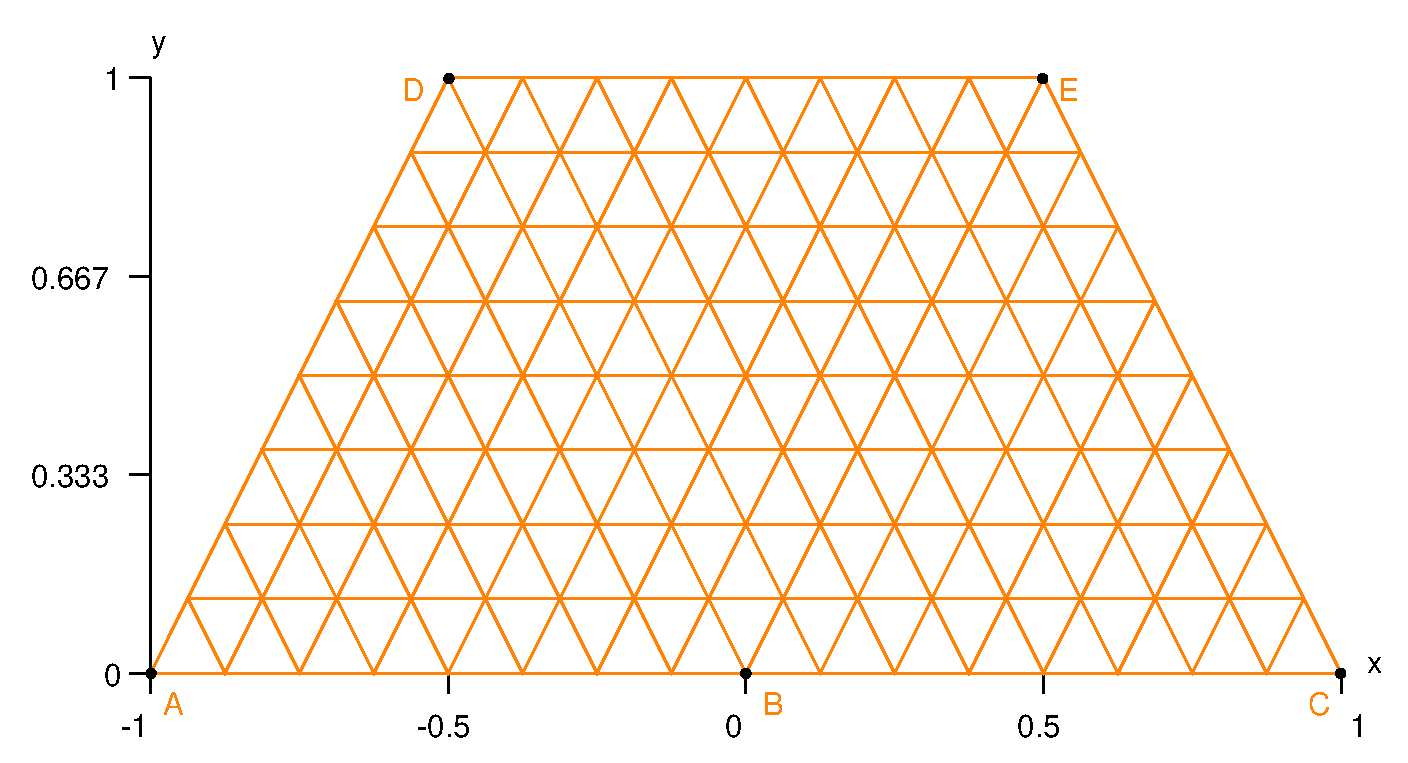
\includegraphics[width=110mm]{three-tri}
  \caption{Mesh obtained by {\small\tt join}ing three triangles}
  \label{\numb section 1.\numb fig 7}
\end{figure}

\begin{Verbatim}[commandchars=\\\{\},formatcom=\small\tt,frame=single,
   label=parag-\ref{\numb section 1.\numb parag 5}.cpp,rulecolor=\color{coment},
   baselinestretch=0.94,framesep=2mm]
   \verm{Cell} \azul{A} ( \textcolor{tag}{tag}::vertex );  x (A) = \laranja{-1.} ;  y (A) = \laranja{0.};
   \verm{Cell} \azul{B} ( \textcolor{tag}{tag}::vertex );  x (B) =  \laranja{0.} ;  y (B) = \laranja{0.};
   \verm{Cell} \azul{C} ( \textcolor{tag}{tag}::vertex );  x (C) =  \laranja{1.} ;  y (C) = \laranja{0.};
   \verm{Cell} \azul{D} ( \textcolor{tag}{tag}::vertex );  x (D) = \laranja{-0.5};  y (D) = \laranja{1.};
   \verm{Cell} \azul{E} ( \textcolor{tag}{tag}::vertex );  x (E) =  \laranja{0.5};  y (E) = \laranja{1.};

   \verm{Mesh} \azul{AB} ( \textcolor{tag}{tag}::segment, A .reverse(), B, \textcolor{tag}{tag}::divided_in, \laranja{8} );
   \verm{Mesh} \azul{BC} ( \textcolor{tag}{tag}::segment, B .reverse(), C, \textcolor{tag}{tag}::divided_in, \laranja{8} );
   \verm{Mesh} \azul{AD} ( \textcolor{tag}{tag}::segment, A .reverse(), D, \textcolor{tag}{tag}::divided_in, \laranja{8} );
   \verm{Mesh} \azul{BD} ( \textcolor{tag}{tag}::segment, B .reverse(), D, \textcolor{tag}{tag}::divided_in, \laranja{8} );
   \verm{Mesh} \azul{BE} ( \textcolor{tag}{tag}::segment, B .reverse(), E, \textcolor{tag}{tag}::divided_in, \laranja{8} );
   \verm{Mesh} \azul{CE} ( \textcolor{tag}{tag}::segment, C .reverse(), E, \textcolor{tag}{tag}::divided_in, \laranja{8} );
   \verm{Mesh} \azul{ED} ( \textcolor{tag}{tag}::segment, E .reverse(), D, \textcolor{tag}{tag}::divided_in, \laranja{8} );

   \verm{Mesh} \azul{ABD} ( \textcolor{tag}{tag}::triangle, AB, BD, AD .reverse() );
   \verm{Mesh} \azul{BCE} ( \textcolor{tag}{tag}::triangle, BC, CE, BE .reverse() );
   \verm{Mesh} \azul{BED} ( \textcolor{tag}{tag}::triangle, BE, ED, BD .reverse() );

   \verm{Mesh} \azul{three_tri} ( \textcolor{tag}{tag}::join, ABD, BCE, BED );
\end{Verbatim}


          %-------------------------------%
\section{~~Mixing triangles and rectangles}\label{\numb section 1.\numb parag 6}
          %-------------------------------%

It is possible to have triangles and quadrilaterals mixed in the same mesh :

\begin{Verbatim}[commandchars=\\\{\},formatcom=\small\tt,frame=single,
   label=parag-\ref{\numb section 1.\numb parag 6}.cpp,rulecolor=\color{coment},
   baselinestretch=0.94,framesep=2mm]
   \verm{Mesh} \azul{ABD} ( \textcolor{tag}{tag}::triangle, AB, BD, AD .reverse() );
   \verm{Mesh} \azul{BCE} ( \textcolor{tag}{tag}::triangle, BC, CE, BE .reverse() );
   \verm{Mesh} \azul{BEFD} ( \textcolor{tag}{tag}::quadrangle, BE, EF, FD, BD .reverse() );
   \verm{Mesh} \azul{two_tri_one_rect} ( \textcolor{tag}{tag}::join, ABD, BEFD, BCE );
\end{Verbatim}

\begin{figure}[ht] \centering
  \psfrag{A}{\small\tt\textcolor{textindraw}{A}}
  \psfrag{B}{\small\tt\textcolor{textindraw}{B}}
  \psfrag{C}{\small\tt\textcolor{textindraw}{C}}
  \psfrag{D}{\small\tt\textcolor{textindraw}{D}}
  \psfrag{E}{\small\tt\textcolor{textindraw}{E}}
  \psfrag{F}{\small\tt\textcolor{textindraw}{F}}
  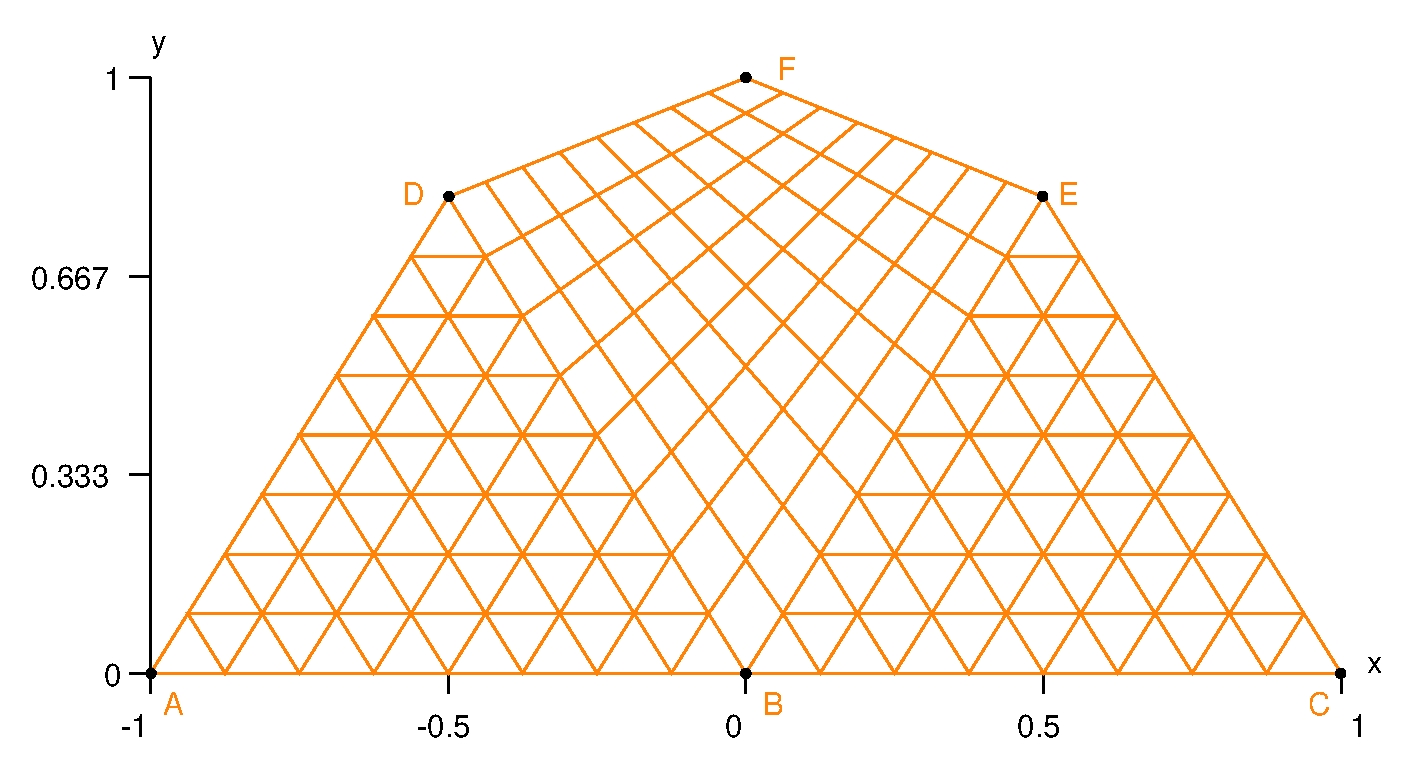
\includegraphics[width=110mm]{two-tri-one-rect}
  \caption{Mixed mesh}
  \label{\numb section 1.\numb fig 8}
\end{figure}

Paragraphs \ref{\numb section 2.\numb parag 2} and \ref{\numb section 2.\numb parag 3}
show other examples of mixed meshes.



